% the following command is only required if the thesis is written in german
\RequirePackage[ngerman=ngerman-x-latest]{hyphsubst}

% change to english for english theses
\documentclass[ngerman,BCOR=1.5cm,twoside]{tudscrreprt}

\usepackage[T1]{fontenc}
\usepackage[utf8]{inputenc}
\usepackage[ngerman]{babel}
\usepackage{isodate}

\usepackage[
    style=numeric-comp,
    backend=biber,
    url=false,
    doi=false,
    isbn=false,
    hyperref,
]{biblatex}
\addbibresource{bibliography.bib}
\AtEveryBibitem{%
    \clearfield{note}%
}

\usepackage[hidelinks]{hyperref} % makes all links clickable but hides ugly boxes
\usepackage[capitalise,nameinlink,noabbrev]{cleveref} % automatically inserts Fig. X in the text with \cref{..}

\usepackage[colorinlistoftodos,prependcaption,textsize=tiny]{todonotes}

\usepackage{graphicx}
\graphicspath{ {./images/} }

% if you need mathy stuff
\newtheorem{lem}{Lemma}
\crefname{lem}{Lemma}{Lemmas}
\newtheorem{thm}{Theorem}
\crefname{thm}{Theorem}{Theorems}
\newtheorem{defs}{Definition}
\crefname{defs}{Def.}{Defs.}

\usepackage{blindtext}

%\usepackage{tudscrsupervisor} % if you want to copy the sources of the task description into the thesis

\usepackage{csquotes}



\usepackage{caption}
\captionsetup{font=sf,labelfont=bf,labelsep=space}
\usepackage{floatrow}
\floatsetup{font=sf}
\floatsetup[table]{style=plaintop}
\captionsetup{singlelinecheck=off,format=hang,justification=raggedright}
\DeclareCaptionSubType[alph]{figure}
\DeclareCaptionSubType[alph]{table}
\captionsetup[subfloat]{labelformat=brace,list=off}

\usepackage{booktabs}
\usepackage{array}
\usepackage{tabularx}
\usepackage{tabulary}
\usepackage{tabu}
\usepackage{longtable}

\usepackage{quoting}

\usepackage[babel]{microtype}

\usepackage{xfrac}

\usepackage{enumitem}
\setlist[itemize]{noitemsep}

\usepackage{ellipsis}
\let\ellipsispunctuation\relax

\usepackage{listings}
\usepackage{inconsolata}
\usepackage{lmodern}

\lstdefinestyle{common-style}{
  basicstyle=\scriptsize\ttfamily,  % the size of the fonts that are used for the code
  showspaces=false,                   % show spaces adding particular underscores
  showstringspaces=false,             % underline spaces within strings
  showtabs=false,                     % show tabs within strings adding particular underscores
%  frame=tlrb,                         % adds a frame around the code
  framexleftmargin=1em,               % space between left part of frame and listing
  tabsize=2,                          % sets default tabsize to 2 spaces
  breaklines=true,                    % sets automatic line breaking
  breakatwhitespace=true,             % sets if automatic breaks should only happen at whitespace
  keywordstyle={\color{blue}\textbf}, % keywords are blue
  commentstyle={\color{gray}},        % comments
  literate={\$}{{{\$}}}1,
  basewidth=0.5em,
  breakindent=40pt,
  breakautoindent=true,
  escapechar=\&,
  aboveskip={0.1\baselineskip}
}

\lstdefinestyle{shortlisting}{
	xleftmargin=\parindent,
	frame=none,
	aboveskip=3pt,belowskip=3pt
}

\lstdefinestyle{unboxed}{
  style=common-style,
	frame=none,
}

% JastAdd
\lstdefinelanguage{AST}{
	style=common-style,
	morekeywords={abstract,rel},
	otherkeywords={::=,->,<,>},
	morecomment=[l]{//}, morecomment=[s]{/*}{*/},
}

\lstdefinelanguage{JRAG}[]{java}{
	style=common-style,
	morekeywords={abstract,public,private,boolean,aspect,null,syn,inh,coll,eq,with,int,contributes,new,return,for,if,else,this,to,true,false},
	morecomment=[l]{//}, morecomment=[s]{/*}{*/},
}

\newcommand{\lstbg}[3][0pt]{{\fboxsep#1\colorbox{#2}{\strut #3}}}
\lstdefinelanguage{diff}[]{java}{
  style=common-style,
  morecomment=[f][\lstbg{HKS07!30}]-,
  morecomment=[f][\lstbg{HKS65!30}]+,
  morecomment=[f][\textit]{@@},
  %morecomment=[f][\textit]{---},
  %morecomment=[f][\textit]{+++},
}

\lstdefinestyle{AST} { language=AST,style=common-style } 
\lstdefinestyle{JRAG} { language=JRAG,style=common-style }
\lstdefinestyle{Java} { language=Java,style=common-style }

\begin{document}

\faculty{Fakultät Informatik}
\department{}
\institute{Institut für Software- und Multimediatechnik}
\chair{Lehrstuhl für Softwaretechnologie}
\title{%
    Entwicklung eines optimalen Verfahrens zur Eroberung des
    Geldspeichers in Entenhausen
}

%% for a bachelor thesis
%\thesis{bachelor}
%\graduation[B.Sc.]{Bachelor of Science}

% for a master thesis
\thesis{master}
\graduation[M.Sc.]{Master of Science}

% for a diploma thesis
%\thesis{diploma}
%\graduation[Dipl.Inf.]{Diplom-Informatiker}

\author{Mickey Mouse}
\emailaddress[]{mickey.mouse@tu-dresden.de}
\matriculationnumber{12345678}
\matriculationyear{2016}
\dateofbirth{1.1.1990}
\placeofbirth{Dresden}
%\discipline{Distributed Systems Engineering}

\course{Distributed Systems Engineering}

\supervisor{%
    Dipl.-Inf. ABC XYZ%
    \and Dr. Sebastian Götz%
}
\professor{Prof. Dr. rer. nat habil. Uwe Aßmann}
\date{10.10.2018}
\maketitle
\newpage

\tableofcontents
\listoffigures
\listoftables

\chapter{Einleitung}\label{ch:introduction}
Thematische Einführung, Motivation

\paragraph{Ziel der Arbeit:} Konzept entwickeln, welches Zonenbasierte MRI mit Kraftsteuerung vereinigt.

Aufbau der Thesis vorstellen

In kommt die Zusammenfassung.

\chapter{Grundlagen}\label{ch:basics}

\section{Figures, Zitate, Mathe}
\begin{figure}[h]
\centering
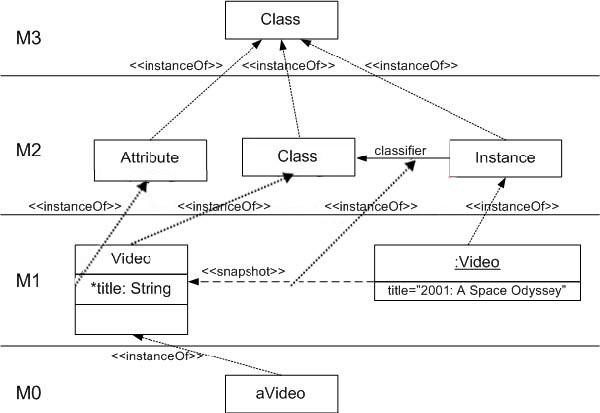
\includegraphics[scale=0.8]{OMG_MOF_4levels}
\caption{Das ist eine schlechte Grafik --- zu viele Pixel. Versuche Vektorgrafiken zu nutzen. Selbst malen geht gut mit draw.io powerpoint
  oder inkscape}\label{fig:mof}
\end{figure}

Wenn eine Abbildung verwendet wird, muss diese immer unbedingt im Text referenziert und beschrieben werden.
Z.B. so: \Cref{fig:mof}.

Zitieren geht so~\cite{haddadin2013towards}.

Math:

$A = \{x | x \in Y\}$

\begin{defs}\label{def:abc}
    A \textbf{Petrinet} is a tuple ${\Sigma = (P, T, F, W)}$.
\end{defs}

Petrinets are defined in~\Cref{def:abc}. See at the head of this document how to create your own definitions/lemma environments.


\subsection{Installation}
\textbf{Windows:} miktex

\textbf{Linux:} texlive-full

\textbf{GUI-Editor} texstudio

Konfiguration vom Editor: Preferences > Build
* default compiler: \emph{latexmk}


\section{Was ist ABC?}

\blindtext

\chapter{Problemanalyse und Modellierung}

\blindtext
\todo[inline]{Write some more}

\begin{lstlisting}[language=AST,label={lst:example-ast},caption={Example AST}]
RailwayContainer ::= Route* Region*;
abstract RailwayElement ::= <Id:int>;
Region : RailwayElement ::= TrackElement* Sensor*;
Semaphore : RailwayElement ::= <Signal:Signal>;
Route : RailwayElement ::= <Active:boolean> SwitchPosition*;
SwitchPosition : RailwayElement ::= <Position:Position>;
Sensor : RailwayElement;
abstract TrackElement:RailwayElement;
Segment : TrackElement ::= <Length:int> Semaphore*;
Switch : TrackElement ::= <CurrentPosition:Position>;
\end{lstlisting}
%
Das Listing~\ref{lst:example-ast} zeigt eine beispielhafte Grammatik, welche im Attribute im folgenden Listing genutzt wird:

\lstinputlisting[language=JRAG,style=unboxed]{code/requiredSensor.jrag}

\chapter{Erprobung der Anwendungsinstallation}\label{ch:evaluation}

\blindtext

\chapter{Zusammenfassung}\label{ch:conclusion}

\blindtext


\printbibliography[heading=bibintoc]\label{sec:bibliography}%

\appendix
\chapter{Weitere Latex-Dokumentation}
\label{ch:appendix}


\confirmation

\end{document}
